\documentclass{article}
\usepackage{graphicx} % Para incluir imágenes
\usepackage[spanish]{babel}
\usepackage{makeidx}
\usepackage{geometry}
\usepackage{graphicx}
\usepackage{caption}
\usepackage{pdfpages}



\geometry{a4paper, total={170mm,257mm}, left=20mm, top=20mm}
\renewcommand{\familydefault}{\sfdefault}


\begin{document}
\begin{titlepage}
    \centering
    \Large
    Universidad Central de Venezuela\\
    Facultad de Ingeniería\\
    Escuela de Ingeniería Eléctrica
    \vspace*{8cm}

    \Huge
    \textbf{Prelaboratorio N° 11: } 

    \textbf{Multivibradores}
    \vfill


    \Large

    Emerson Warhman \\
    C.I. 25.795.480 \\
    \today

\end{titlepage}
\tableofcontents
\newpage

\section{Introducción}

\section{Introducción}

En el ámbito de la electrónica, los amplificadores operacionales son componentes fundamentales que se utilizan en una amplia variedad de aplicaciones, desde sistemas de audio hasta equipos de medición y control. Un amplificador operacional es un dispositivo de alta ganancia con dos entradas y una salida, que puede amplificar señales de voltaje muy pequeñas.

El objetivo de este informe de laboratorio es analizar el comportamiento y las características de un amplificador operacional en sus etapas diferencial, impulsora y de potencia y del circuito multietapas en diferentes conilustraciónciones. Se realizarán mediciones de los puntos estáticos, modelos dinámicos, ganancia respuesta en frecuencia y utilizando circuitos con realimentación negativa y positiva.  


\section{Resumen}

\section{Marco teorico}

\section{Metodología}

\section{Resultados}

\section{Análisis de resultados}

\section{Conclusiones}

\section{Anexos}

\begin{figure}[ht]
    \centering
    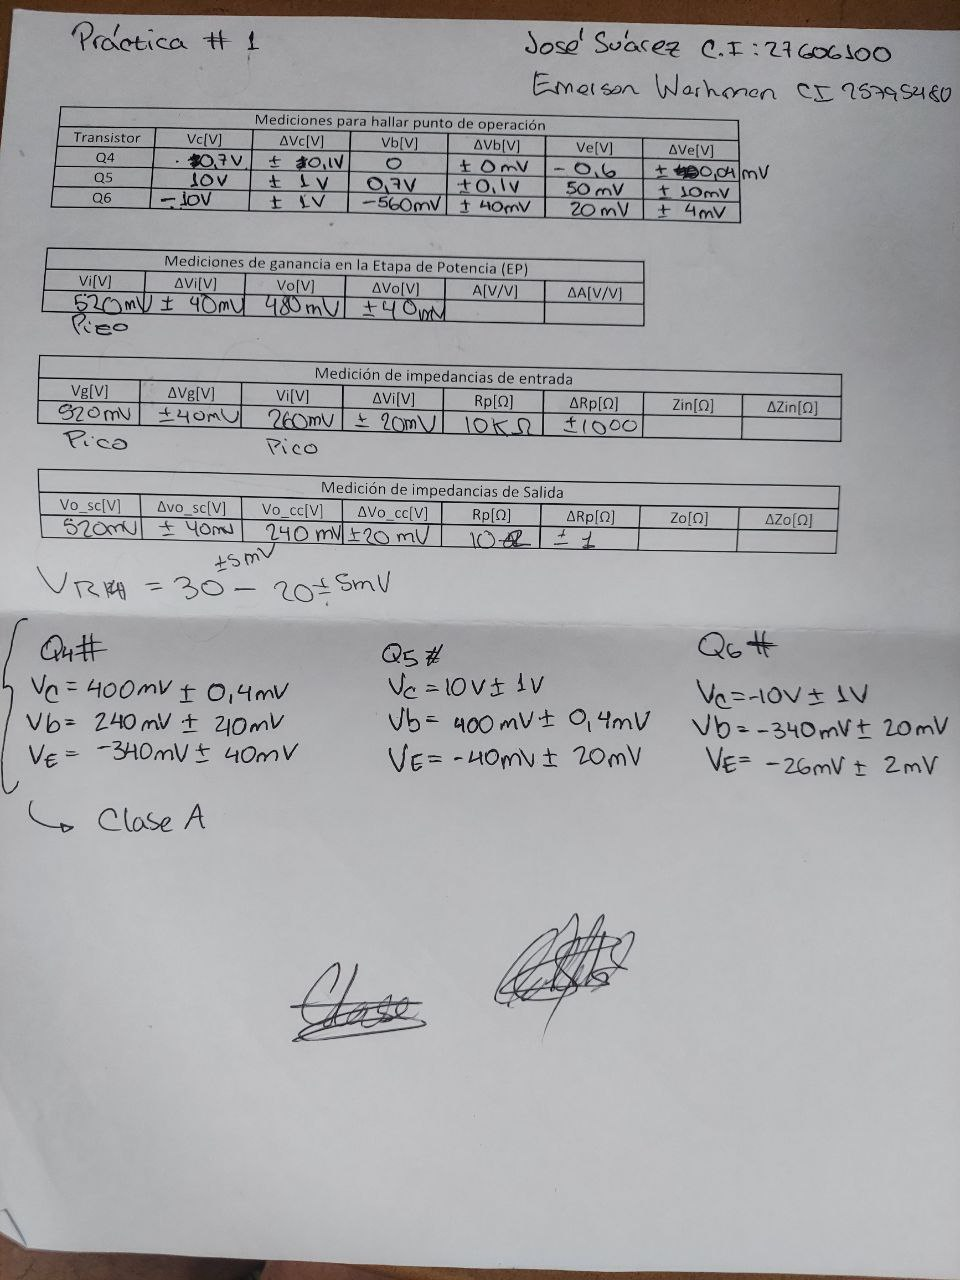
\includegraphics[width=1.0\textwidth]{src/images/p1/p1-hoja-de-datos.jpg}
    \caption{Hoja de datos práctica N° 1}
    \label{fig:hoja-de-datos-p1}
\end{figure}

\begin{figure}[ht]
    \centering
    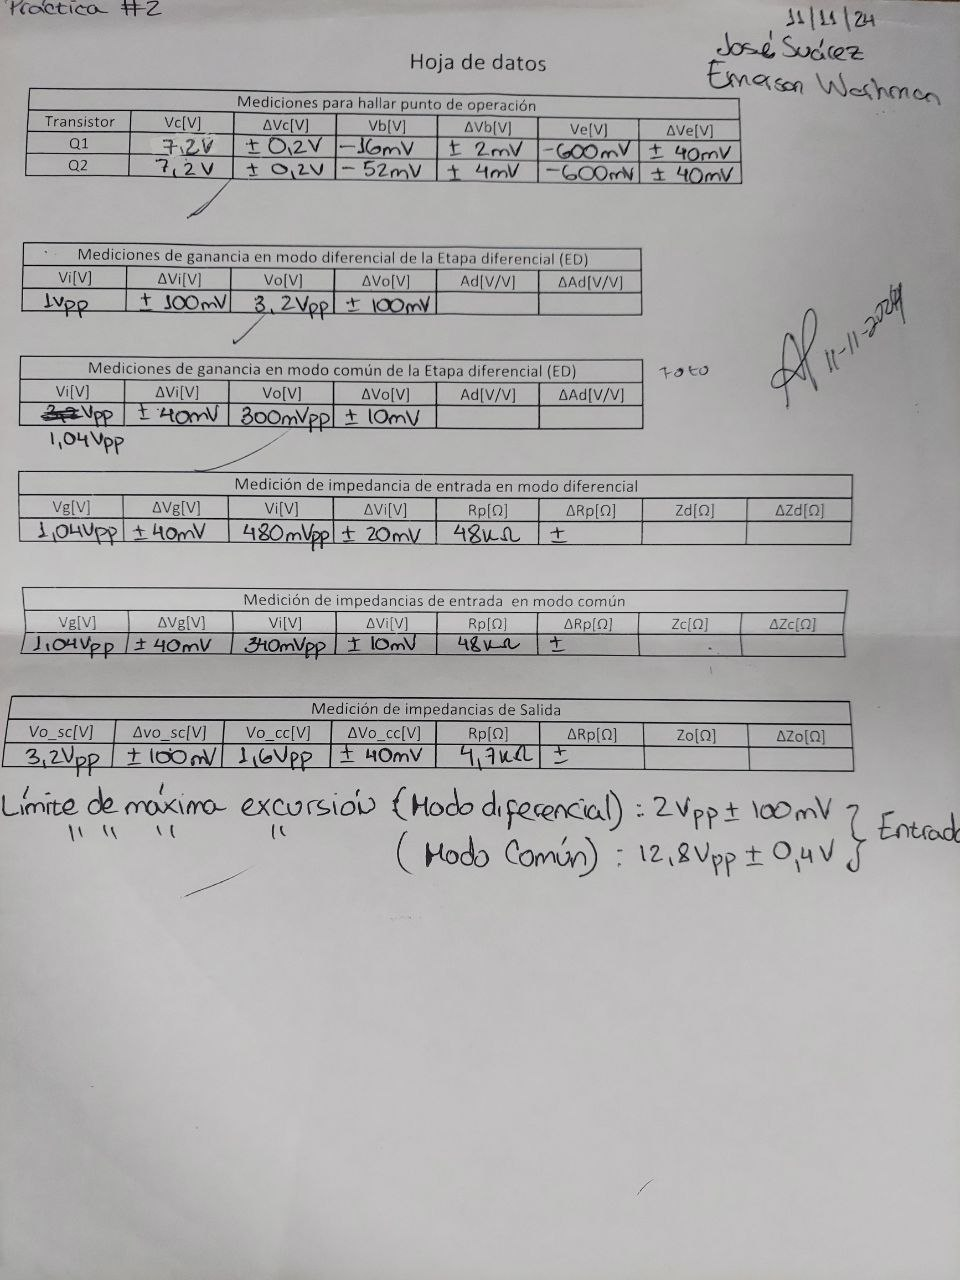
\includegraphics[width=1.0\textwidth]{src/images/p2/p2-hoja-de-datos.jpg}
    \caption{Hoja de datos práctica N° 2}
    \label{fig:hoja-de-datos-p2}
\end{figure}

\begin{figure}[ht]
    \centering
    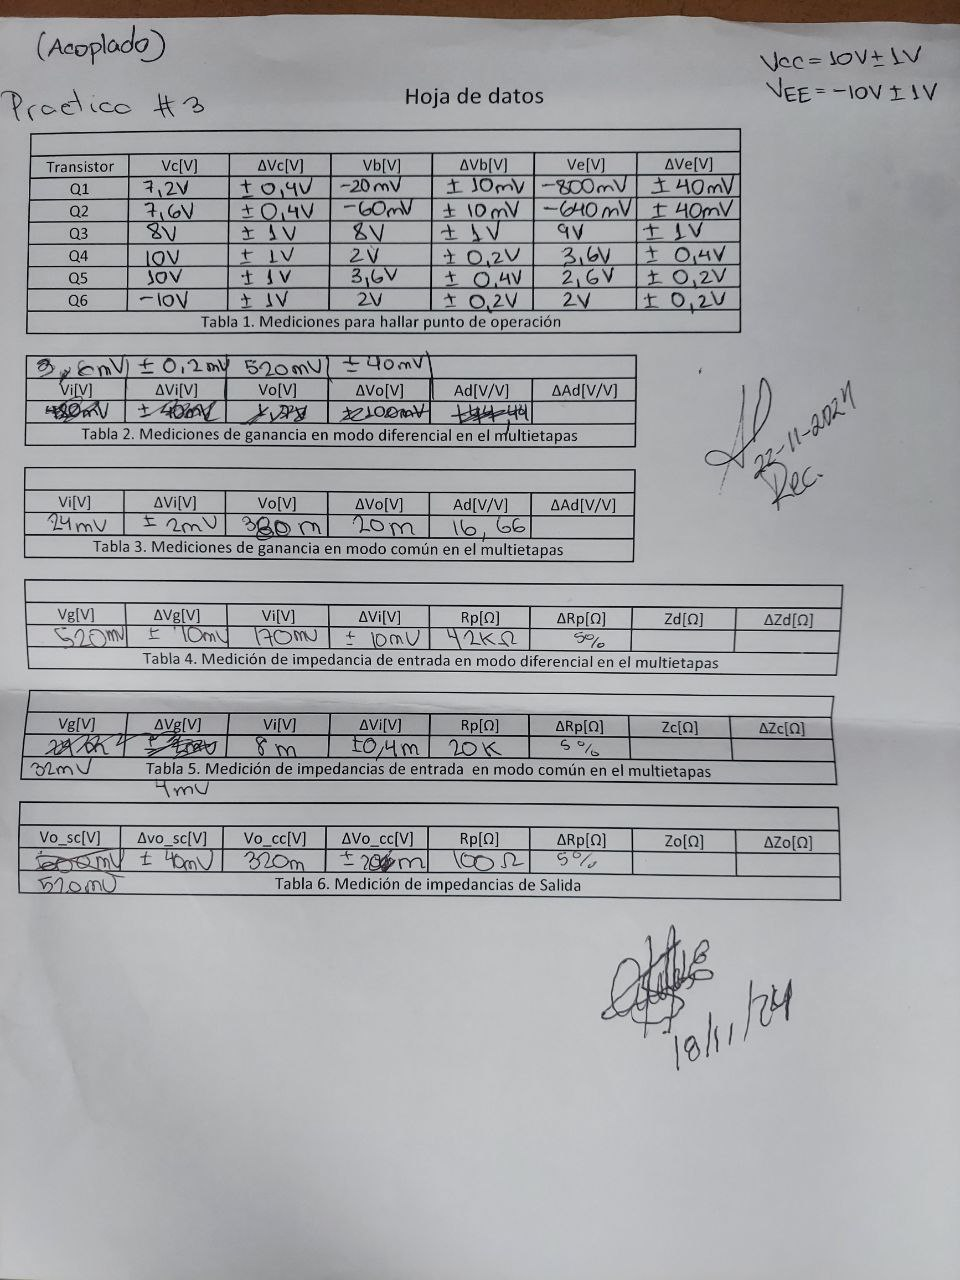
\includegraphics[width=1.0\textwidth]{src/images/p3/p3-hoja-de-datos.jpg}
    \caption{Hoja de datos práctica N° 3-1}
    \label{fig:hoja-de-datos-p3-1}
\end{figure}

\begin{figure}[ht]
    \centering
    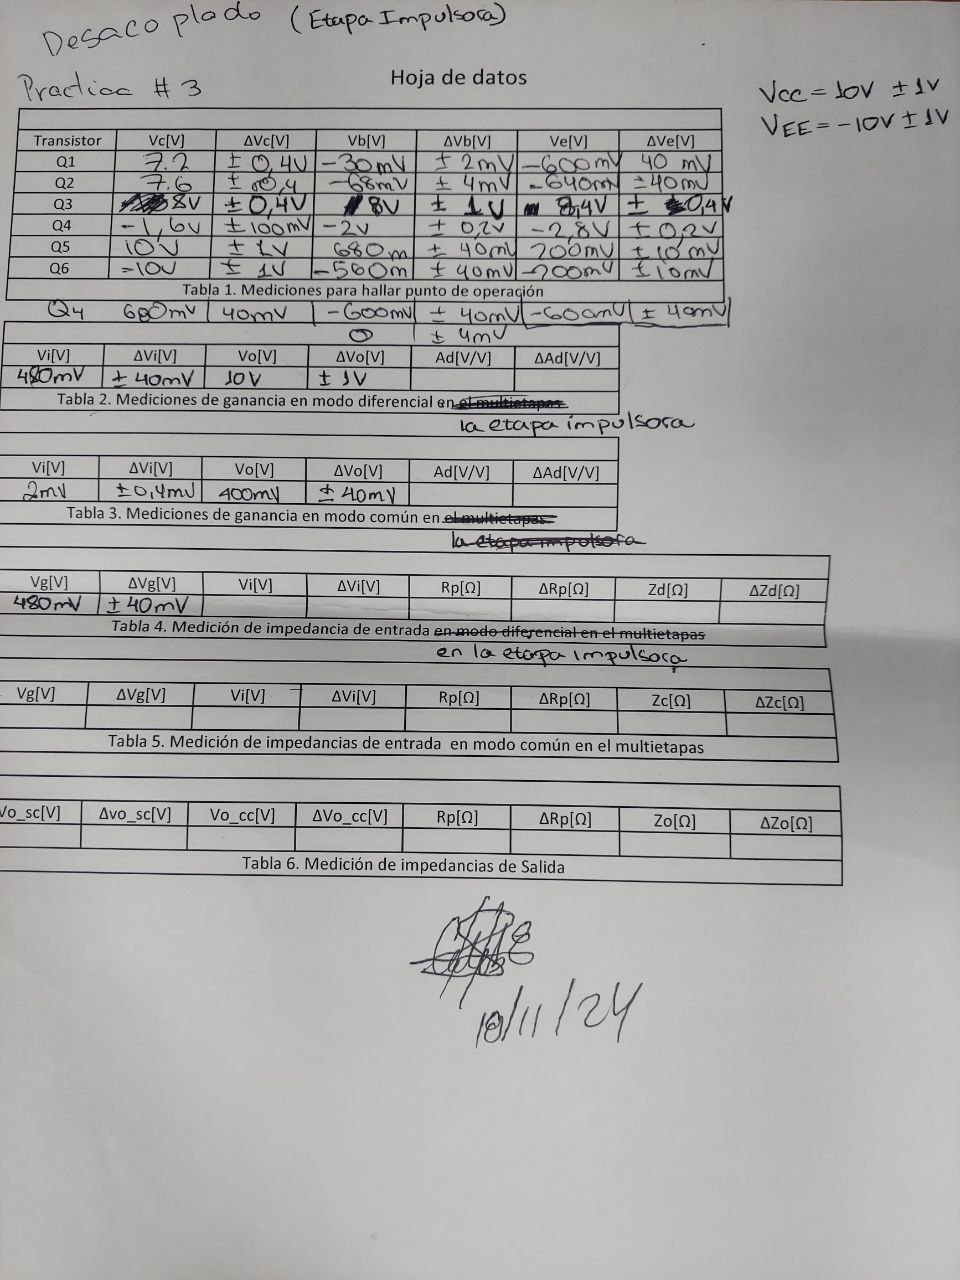
\includegraphics[width=1.0\textwidth]{src/images/p3/p3-hoja-de-datos-2.jpg}
    \caption{Hoja de datos práctica N° 3-2}
    \label{fig:hoja-de-datos-p3-2}
\end{figure}

\begin{figure}[ht]
    \centering
    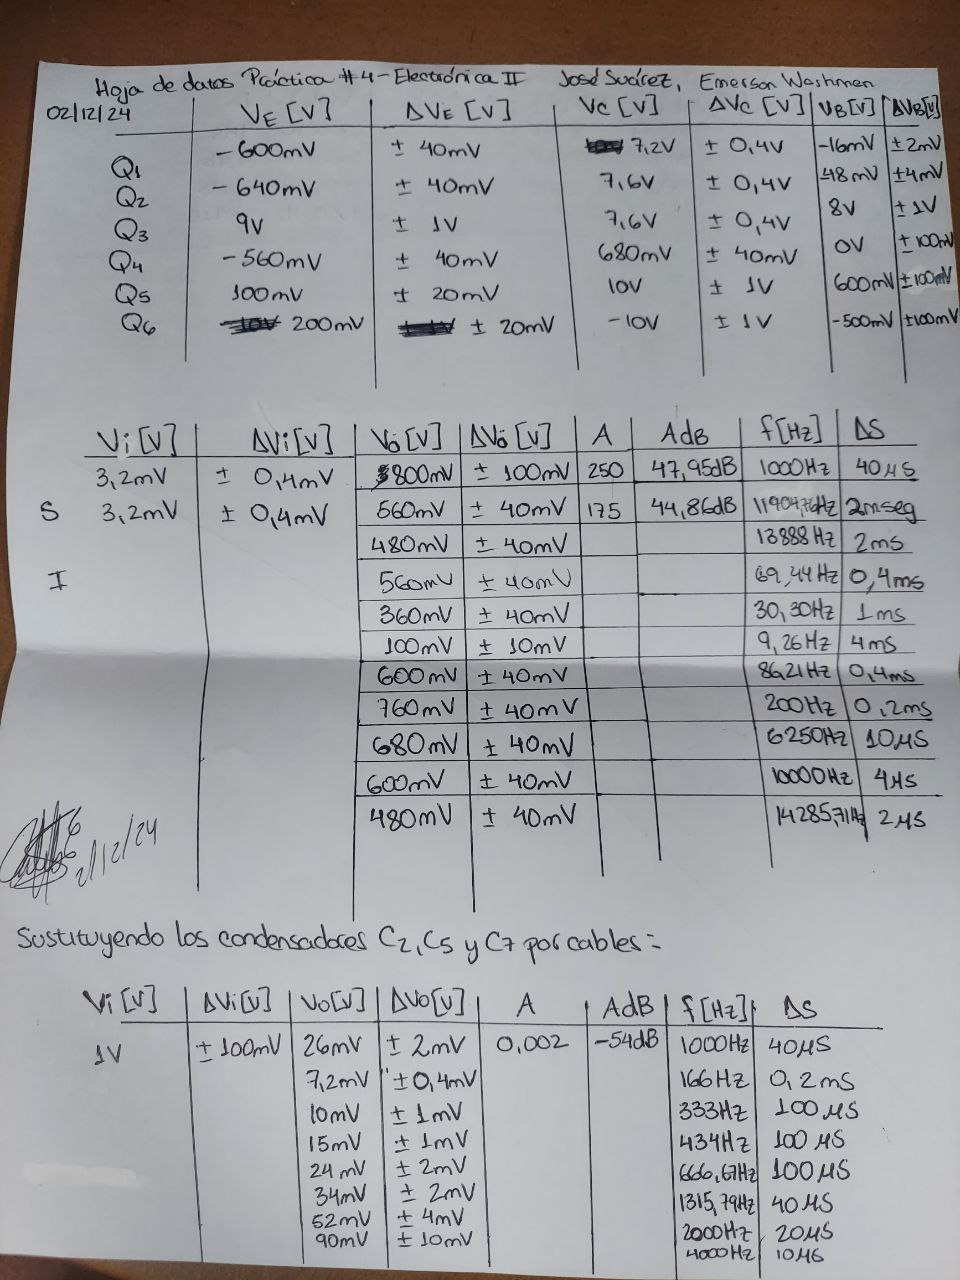
\includegraphics[width=1.0\textwidth]{src/images/p4/p4-hoja-de-datos-1.jpg}
    \caption{Hoja de datos práctica N° 4-1}
    \label{fig:hoja-de-datos-p4-1}
\end{figure}

\begin{figure}[ht]
    \centering
    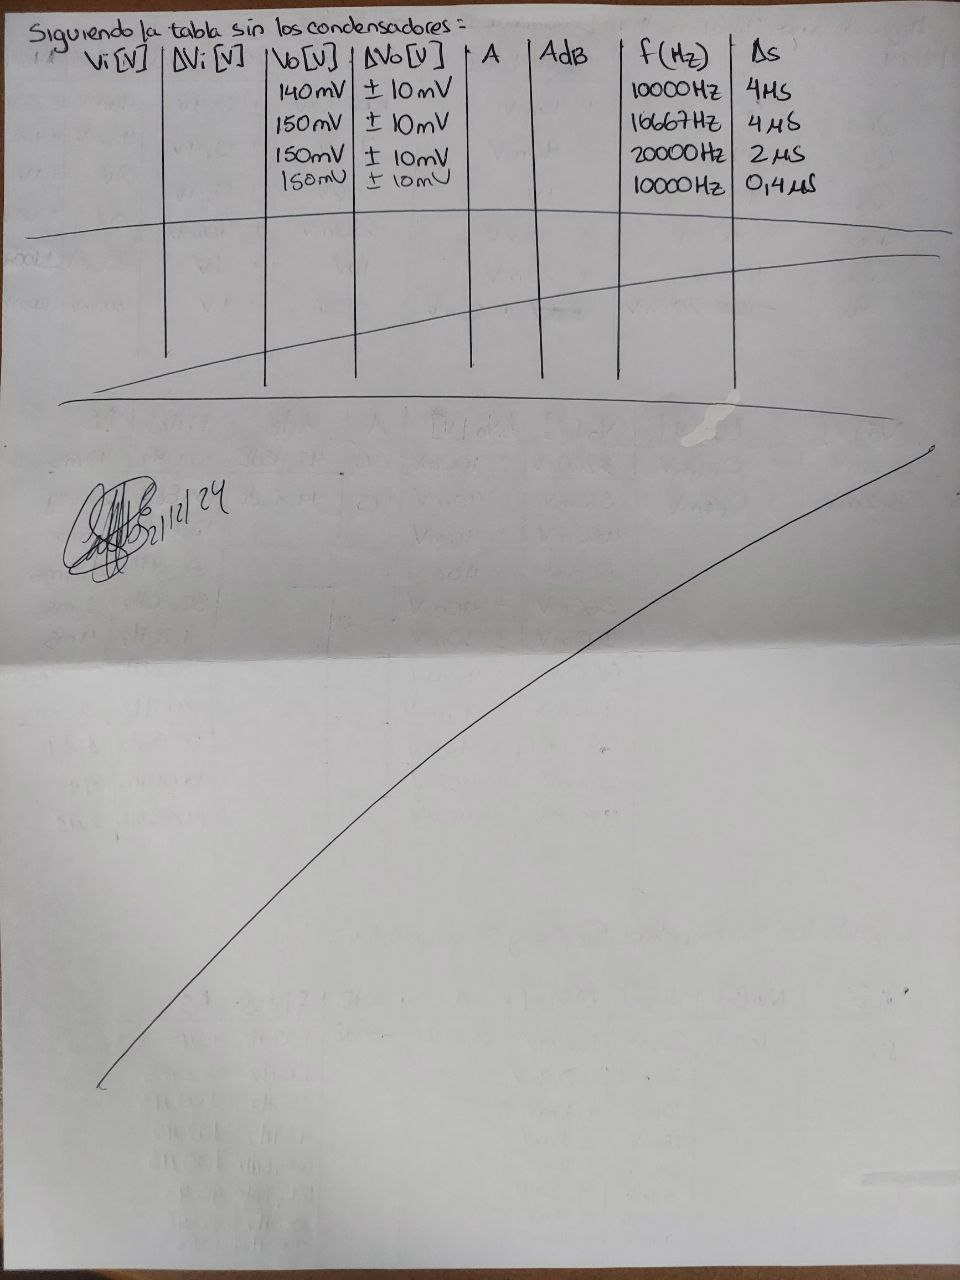
\includegraphics[width=1.0\textwidth]{src/images/p4/p4-hoja-de-datos-2.jpg}
    \caption{Hoja de datos práctica N° 4-2}
    \label{fig:hoja-de-datos-p4-2}
\end{figure}

\begin{figure}[ht]
    \centering
    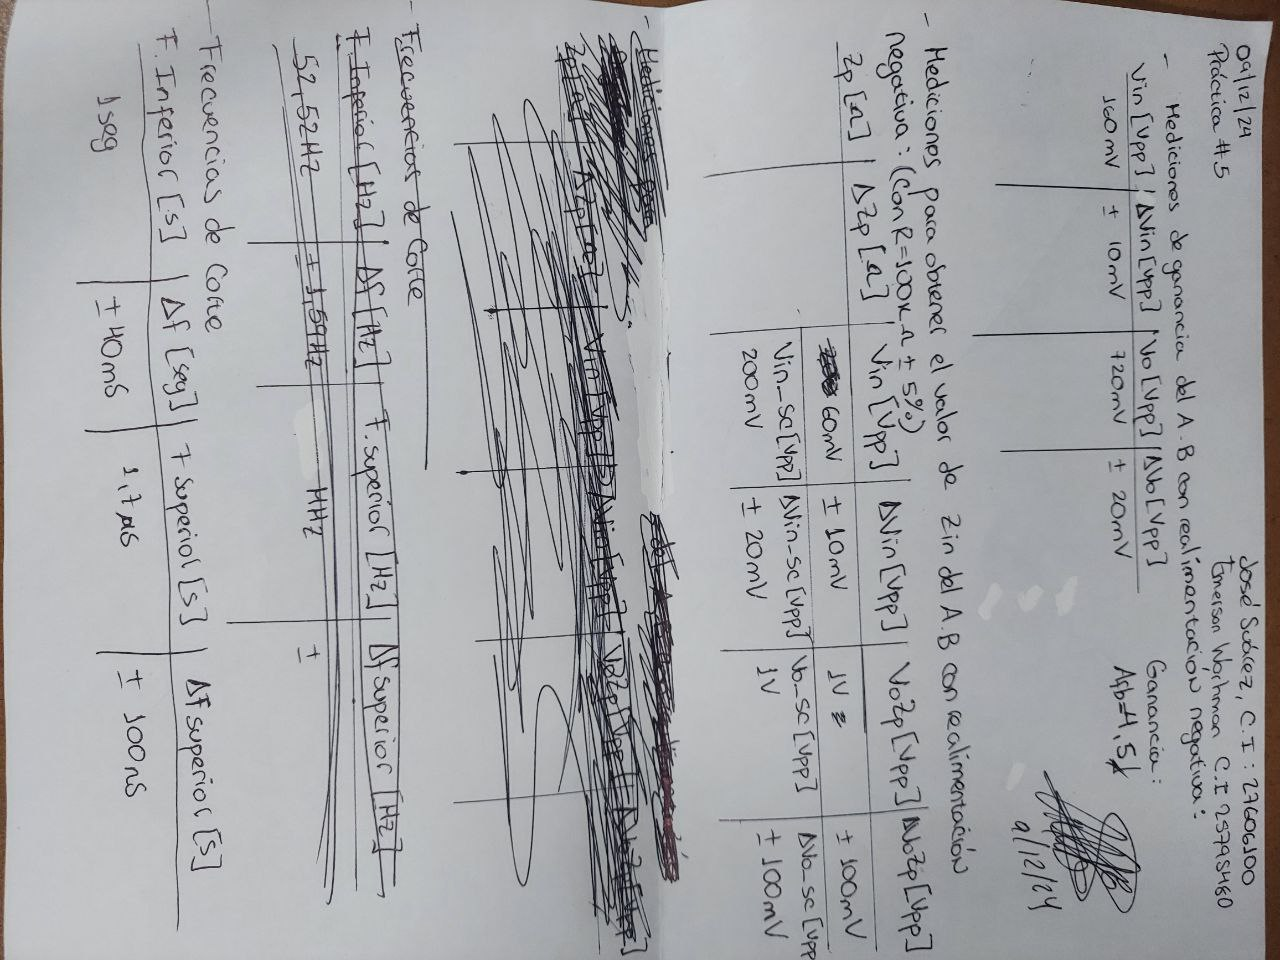
\includegraphics[width=1.0\textwidth, angle=90]{src/images/p5/p5-hoja-de-datos-1.jpg}
    \caption{Hoja de datos práctica N° 5-1}
    \label{fig:hoja-de-datos-p5-1}
\end{figure}

\begin{figure}[ht]
    \centering
    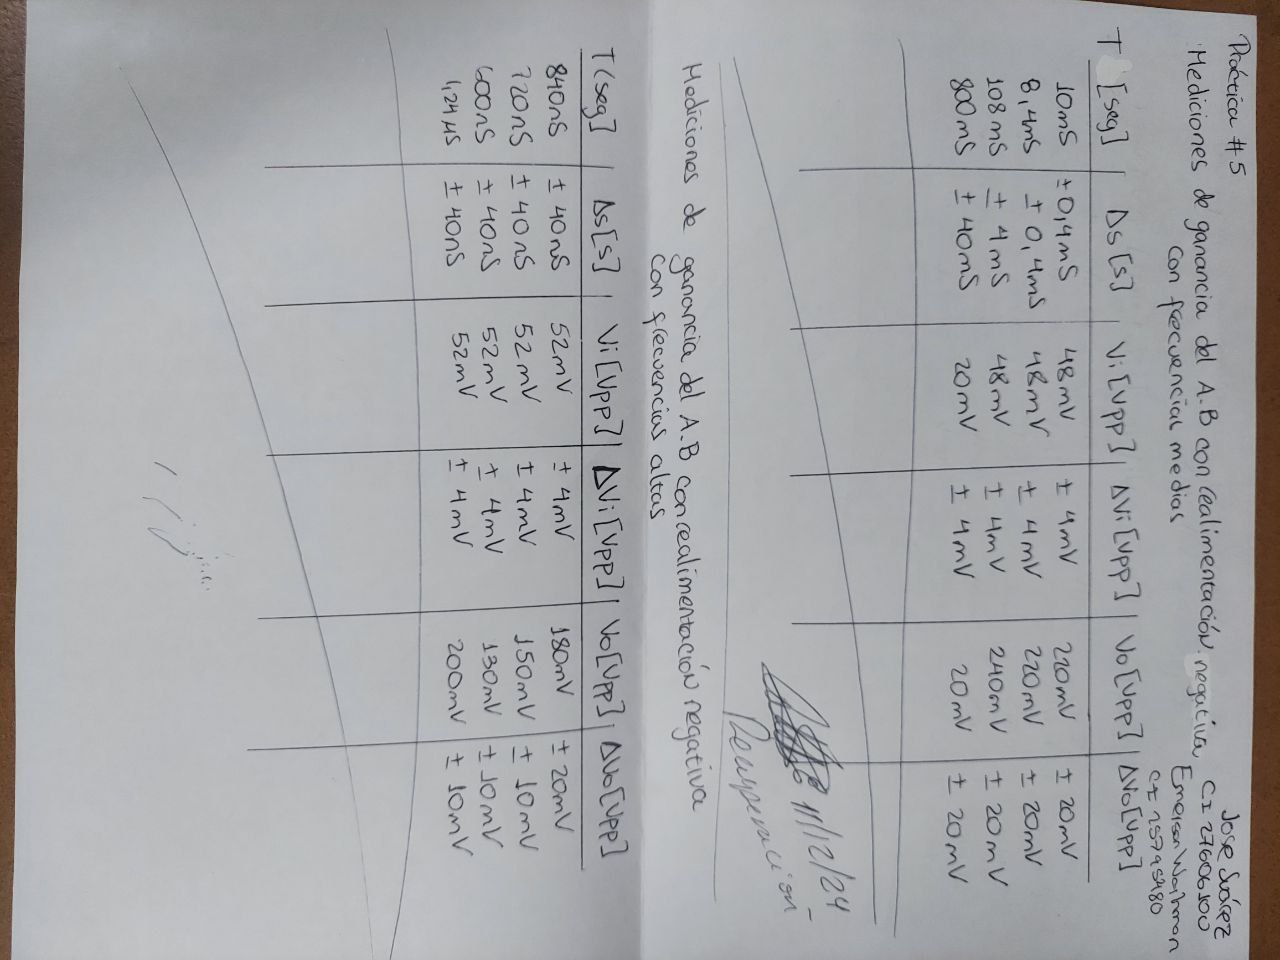
\includegraphics[width=1.0\textwidth,angle=90]{src/images/p5/p5-hoja-de-datos-2.jpg}
    \caption{Hoja de datos práctica N° 5-2}
    \label{fig:hoja-de-datos-p5-2}
\end{figure}

\begin{figure}[ht]
    \centering
    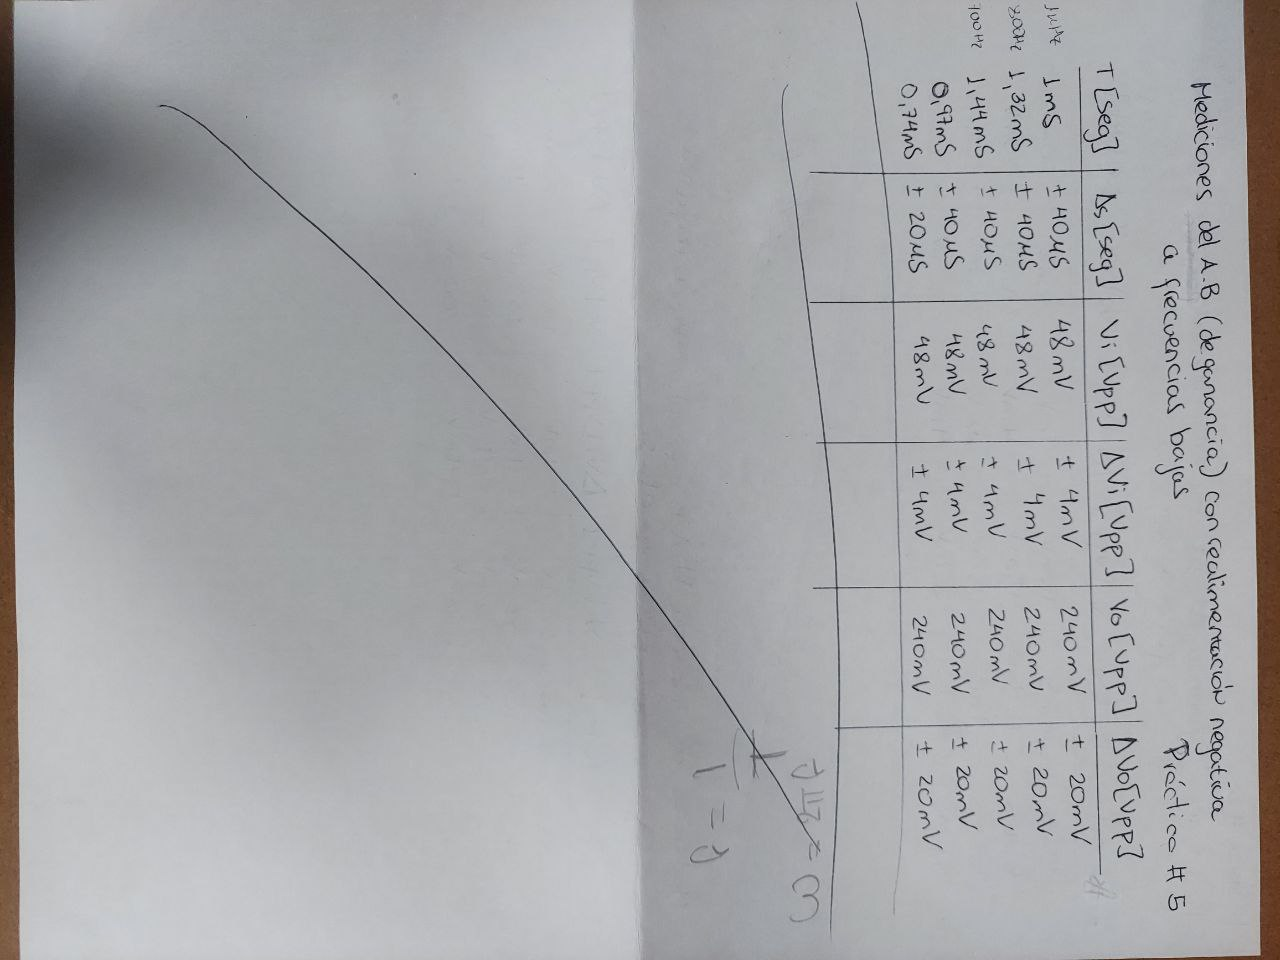
\includegraphics[width=1.0\textwidth, angle=90]{src/images/p5/p5-hoja-de-datos-3.jpg}
    \caption{Hoja de datos práctica N° 5-3}
    \label{fig:hoja-de-datos-p5-3}
\end{figure}

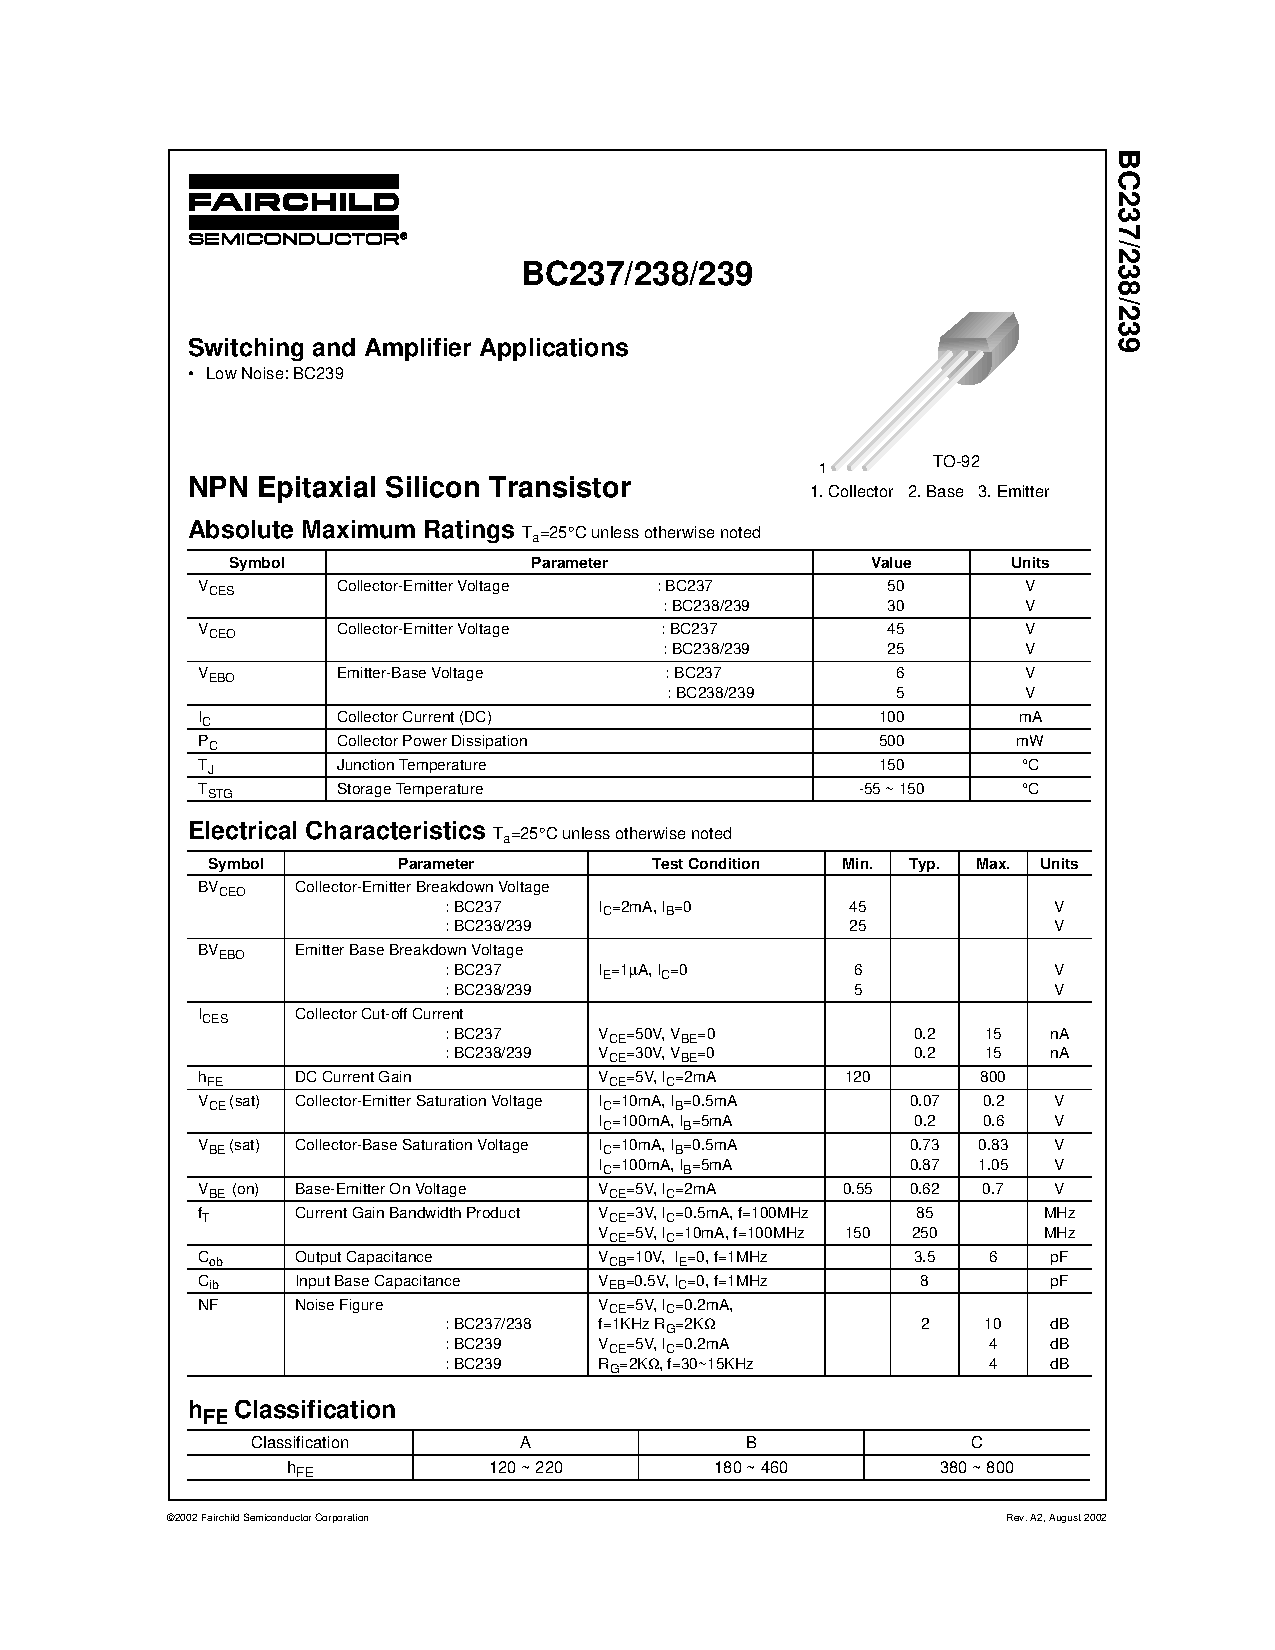
\includepdf[page=-, width=0.9\textwidth]{src/assets/BC237.pdf}
\captionof{figure}{Hoja de datos del transistor BC237}

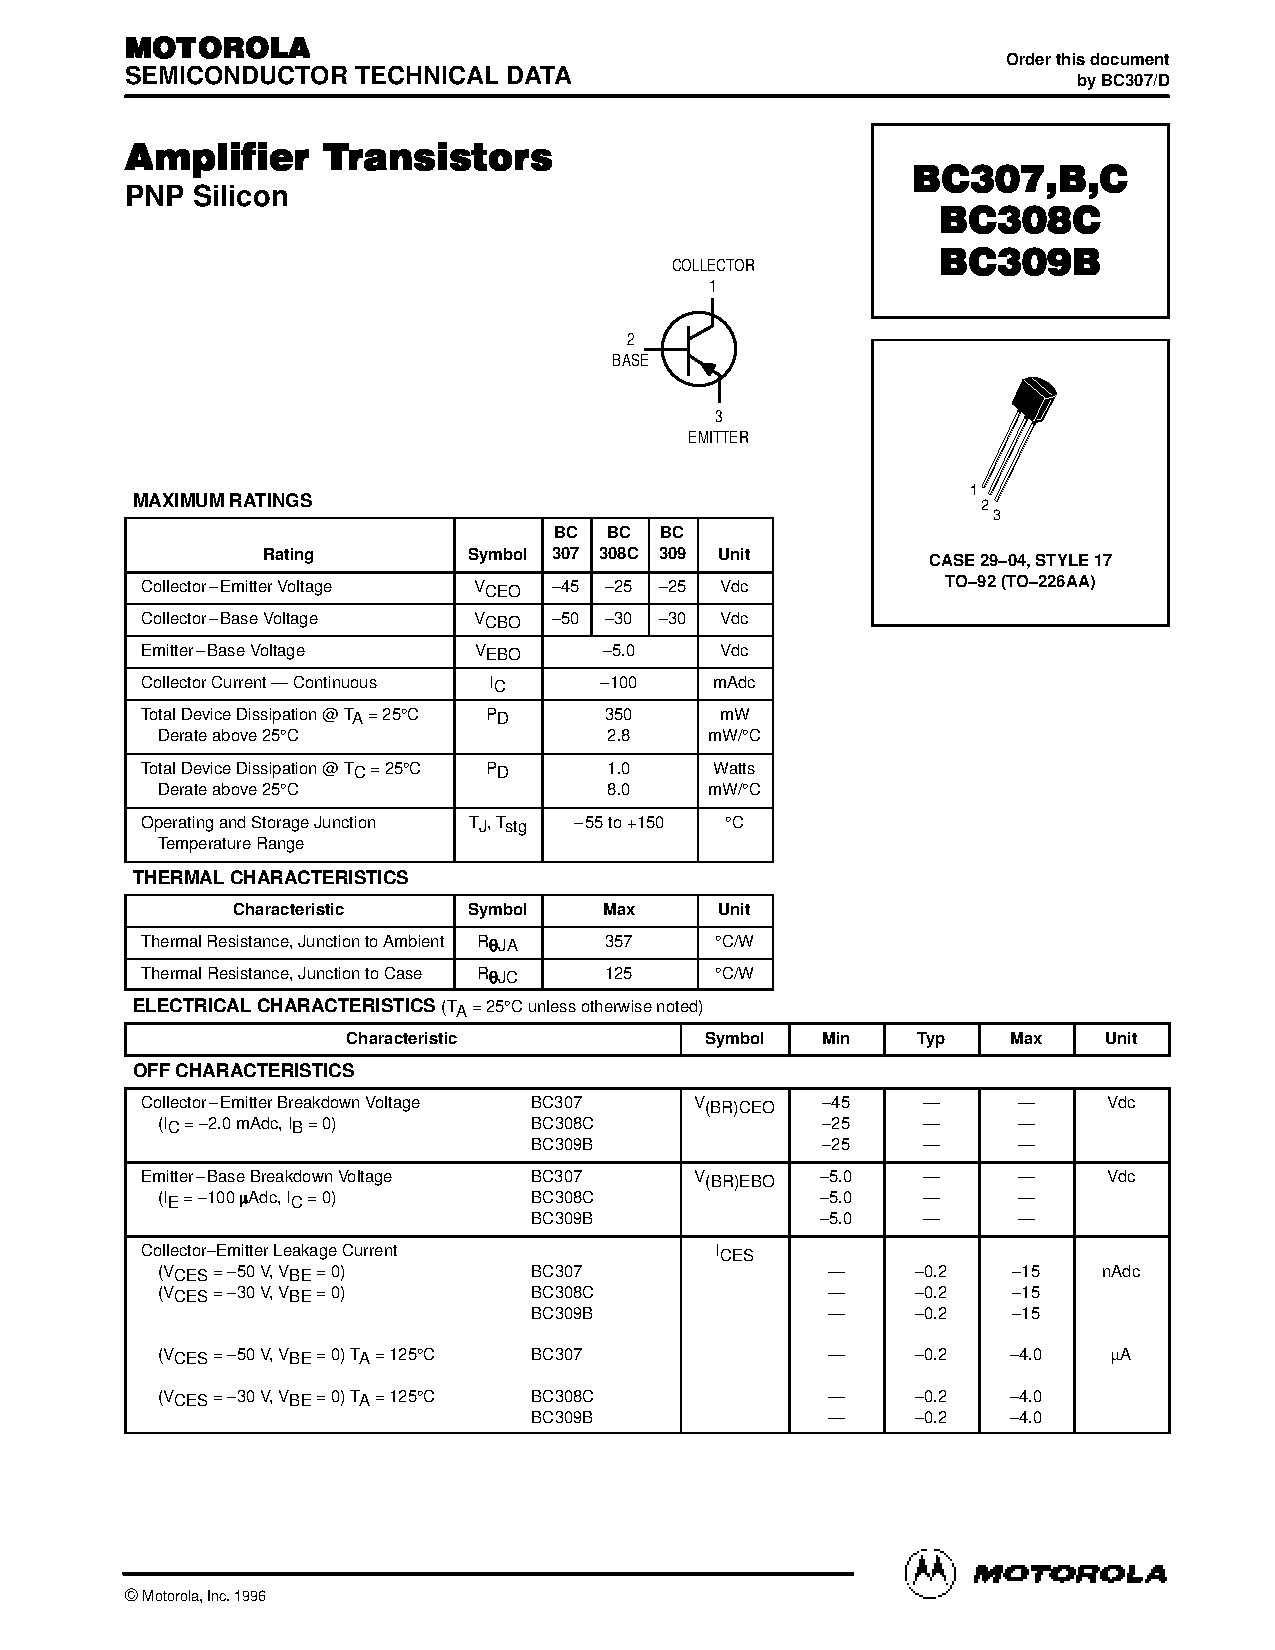
\includepdf[page=-, width=0.9\textwidth]{src/assets/bc307.pdf}
\captionof{figure}{Hoja de datos del transistor BC307}


\end{document}
